\chapter{Слежение и компенсация}
\label{ch:chap5}

\section{Решение задачи компенсации}
Зададим сигнал $f$ в модели
\begin{equation}
    \begin{cases}
       \dot{x} = Ax + Bu + Df,\\
     y=Cx,  
    \end{cases}
\end{equation}

виде суммы гармоник

\begin{equation}
    f(t) = \sum \limits_{k=1}^5 A_k \sin(\omega_kt+\phi_k),
\end{equation}
где
\begin{equation}
    \begin{matrix}
        A_1 = 1, & \omega_1 = 0.5, & \phi_1 = 0\\
        A_2 = 0.8, & \omega_2 = 1, & \phi_2 = \pi /4\\
        A_3 = 0.6, & \omega_3 = 1.5, & \phi_3 = \pi /3\\
        A_4 = 0.4, & \omega_4 = 2, & \phi_4 = -\pi/4\\
        A_5= 0.2, & \omega_5 = 2.5, & \phi_5 = \pi / 6\\
    \end{matrix}
\end{equation}

Построим компенсирующий регулятор, гарантирующий выполнение условия

\begin{equation}
\label{5_goal_1}
    \lim \limits_{t \to \infty} \| \varphi(t) \| = 0,
\end{equation}



Запишем возмущение $f$ через генератор

\begin{equation}
    \begin{cases}
        \dot{w} = \Gamma_f w\\
        f = Y_fw
    \end{cases}
\end{equation}
Теперь нам необходимо определить значения $\Gamma_f$, $Y_f$ и $w(0)$

\begin{multline}
    \Gamma_f = block \,diag \left( 
    \begin{bmatrix}
        0 & -w_1\\
        w_1 & 0
    \end{bmatrix}\dots 
    \begin{bmatrix}
        0 & -w_5\\
        w_5 & 0
    \end{bmatrix}
    \right) =\\[2ex]
    = \begin{bmatrix}
        0 & -0.5 & 0 & 0 & 0 & 0 & 0 & 0&0&0\\
        0.5 & 0 & 0 & 0 & 0 & 0 & 0 & 0&0&0\\
        0 & 0 & 0 & -1 & 0 & 0 & 0 & 0&0&0\\
        0 & 0 & 1 & 0 & 0 & 0 & 0 & 0&0&0\\
        0 & 0 & 0 & 0 & 0 & -1.5 & 0 & 0&0&0\\
        0 & 0 & 0 & 0 & 1.5 & 0 & 0 & 0&0&0\\
        0 & 0 & 0 & 0 & 0 & 0 & 0 & -2&0&0\\
        0 & 0 & 0 & 0 & 0 & 0 & 2 & 0&0&0\\
        0 & 0 & 0 & 0 & 0 & 0 & 0 & 0&0&-2.5\\
        0 & 0 & 0 & 0 & 0 & 0 & 0 & 0&2.5&0
    \end{bmatrix} 
\end{multline}

При переходе к матричной экспоненте $e^{\Gamma_f t}$ каждый блок 

\begin{equation}\begin{bmatrix}
        0 & -w_i\\
        w_i & 0
\end{bmatrix}\end{equation}
перейдет в 
\begin{equation}\begin{bmatrix}
        \cos (w_it) & -\sin (w_it)\\
        \sin (w_it) & \cos (w_it)
\end{bmatrix}
\end{equation}
    
Запишем $f(t)$ и упростим его компоненты
\begin{multline}
    f(t) = \sin (0.5t) + 0.8 \sin(t+\pi/4)+ 0.6 \sin (1.5 t+ \pi/3)+\\+0.4 sin(2t-\pi/4) + 0.2\sin(2.5t+\pi/6) =\sin (0.5t)+ 0.4\sqrt{2} \sin{t} +\\+ 0.4\sqrt{2} \cos{t} + 0.3 \sin(1.5t)+
    0.3 \sqrt{3} \cos(1.5t) + 0.2 \sqrt{2} \sin(2t) - \\-0.2\sqrt{2}\cos(2t) + 0.1 \sqrt{3} \sin(2.5t) + 0.1 \cos(2.5t)
\end{multline}
Основываясь на следующей системе уравнений, найдем подходящие значения $w(0)$ и $Y_f$

\begin{equation}
\begin{cases}
    w = e^{\Gamma_f t} w(0)\\
    f = Y_f e^{\Gamma_f t} w(0)
\end{cases}
\end{equation}

\begin{equation}
    w(0) = \begin{bmatrix}
       1 &  0 & 1 & 0 & 1 & 0 & 1 & 0 & 1 & 0
    \end{bmatrix}^T
\end{equation}

\begin{equation}
    Y_f = \begin{bmatrix}
        0 & 1 & 0.4\sqrt{2} & 0.4\sqrt{2} & 0.3\sqrt{3} & 0.3 & -0.2 \sqrt{2} & 0.2 \sqrt{2} & 0.1 & 0.1 \sqrt{3}
    \end{bmatrix}
\end{equation}

Запишем общий вид необходимого регулятора

\begin{equation}
    u = Kx + K_f w
\end{equation}

В качестве $K$ возьмем ранее вычисленный в пункте 4.1 регулятор 
\begin{equation}
    K = \begin{bmatrix}
        3064 & 4364 & -26684 & -11174
    \end{bmatrix}
\end{equation}

теперь нам необходимо вычислить компенсирующую компоненту $K_f$ регулятора. Запишем систему матричных уравнений Франкиса-Дэвисона

\begin{equation}
\label{5_fran_f}
    \begin{cases}
       P_f \Gamma_f - (A+BK)P_f-DY_f=BK_f\\
       CP_f = 0
    \end{cases}
\end{equation}

Проверим условие существования решения системы уравнений (\ref{5_fran_f}).

Решение относительно $P_f$ и $K_f$ есть, если

\begin{equation}
\label{5_f_rule}
    rank \begin{bmatrix}
        A+BK-I\lambda_{i\Gamma_f}&B\\
        C & 0
    \end{bmatrix} = \text{число строк}
\end{equation}

В ходе проверки этого условия было выяснено, что ранг искомых матриц равен 5, что меньше числа строк в матрицах, 6. От нас требуется компенсировать только значение угла (\ref{5_goal_1}), то есть $y_2(t) = \varphi(t)$. Будем работать с матрицей $\tilde{C}$ вместо $C$

\begin{equation}
    C = \begin{bmatrix}
        1 & 0 & 0 & 0\\
        0 & 0 & 1 & 0
    \end{bmatrix} \Rightarrow 
    \tilde{C} =\begin{bmatrix}
        0 & 0 & 1 & 0
    \end{bmatrix} 
\end{equation}

Вновь проверим, условие (\ref{5_f_rule}) только теперь вместо матрицы $C$ будем использовать $\tilde{C}$. Условие существования решения выполнено ранг каждой исследованной матрицы равен 5, что совпадает с количеством строк в матрицах.

В результате решения системы (\ref{5_fran_f}) получим значение компенсирующей компоненты регулятора

\begin{equation}
    K_f = \begin{bmatrix}
        -736.0530	\\-1056.7\\-367.4171	\\48.9573	\\-145.2753	\\86.1095	\\-27.2456	\\-76.8480	\\-31.9406	\\3.5614
    \end{bmatrix}^T
\end{equation}

Проведем моделирование для линейной модели 

\begin{figure}[!h]
\center{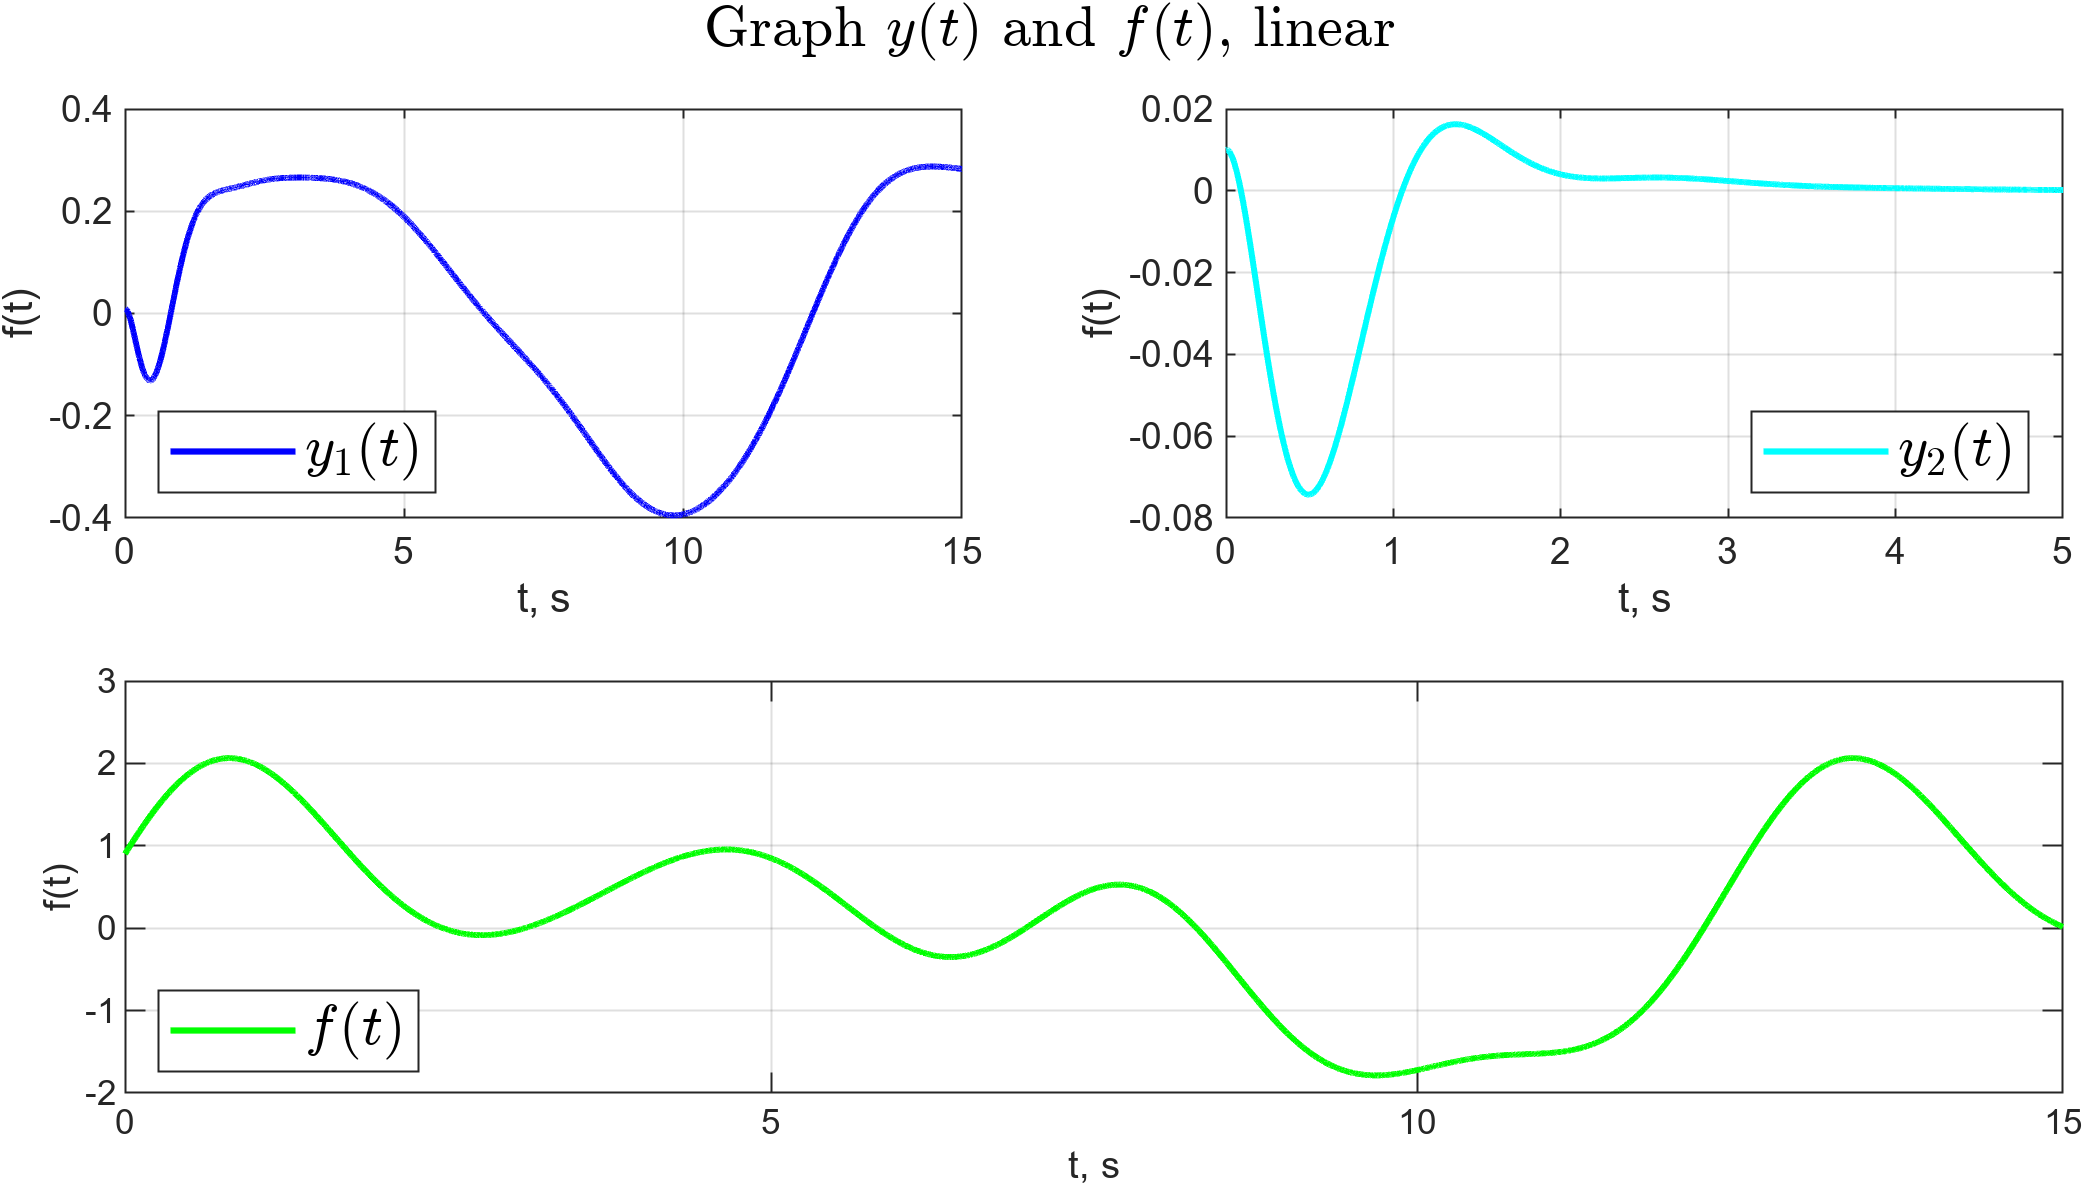
\includegraphics[width=1\linewidth]{pic2/5_f_lin.png}}
\caption{Графики выходного сигнала $y(t)$ и внешнего воздействия $f(t)$ для линейной системы.}
\label{5_f_lin}
\end{figure}

Заметим, что целевое условие (\ref{5_goal_1}) действительно выполнено, компонента выхода $y_2(t) = \varphi(t)$ сходится к нулю с течение времени. Задача компенсации для линейной системы выполнена.

Исследуем поведение регулятора для нелинейного случая.

\begin{figure}[!h]
\center{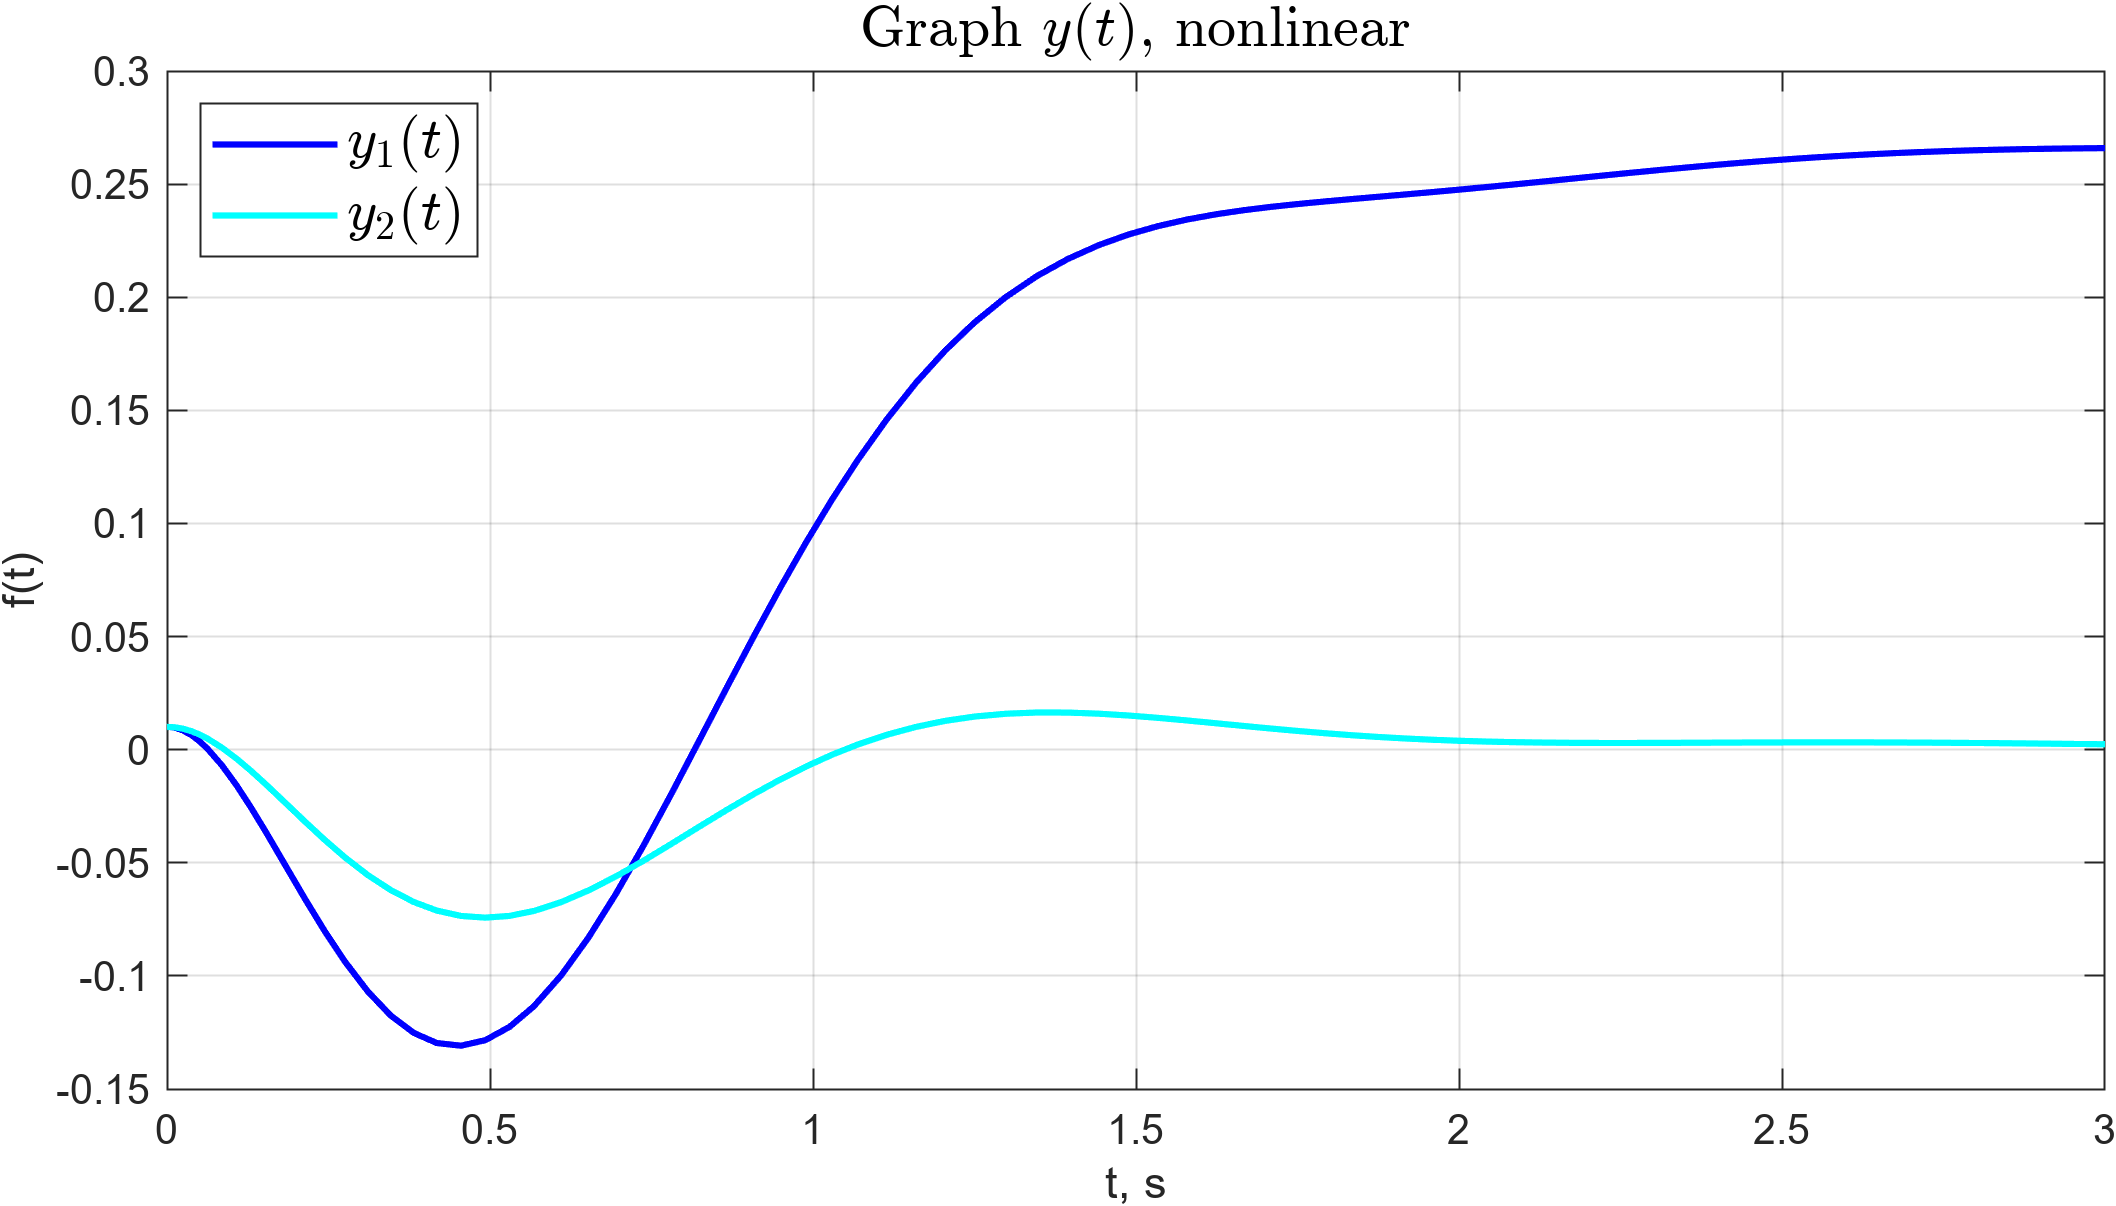
\includegraphics[width=1\linewidth]{pic2/5_f_nonlin.png}}
\caption{График выходного сигнала $y(t)$ для нелинейной системы при $x(0) = 
    [0.01 \,\, 0.01 \,\, 0.01 \,\, 0.01]^T$.}
\label{5_f_nonlin}
\end{figure}

Для нелинейного случая при начальных условиях системы $x(0) = \begin{bmatrix}
    0.01 & 0.01 & 0.01 & 0.01
\end{bmatrix}^T$ синтезированный компенсирующий регулятор так же справляется с задачей (рисунок \ref{5_f_nonlin}).

\begin{figure}[!h]
\center{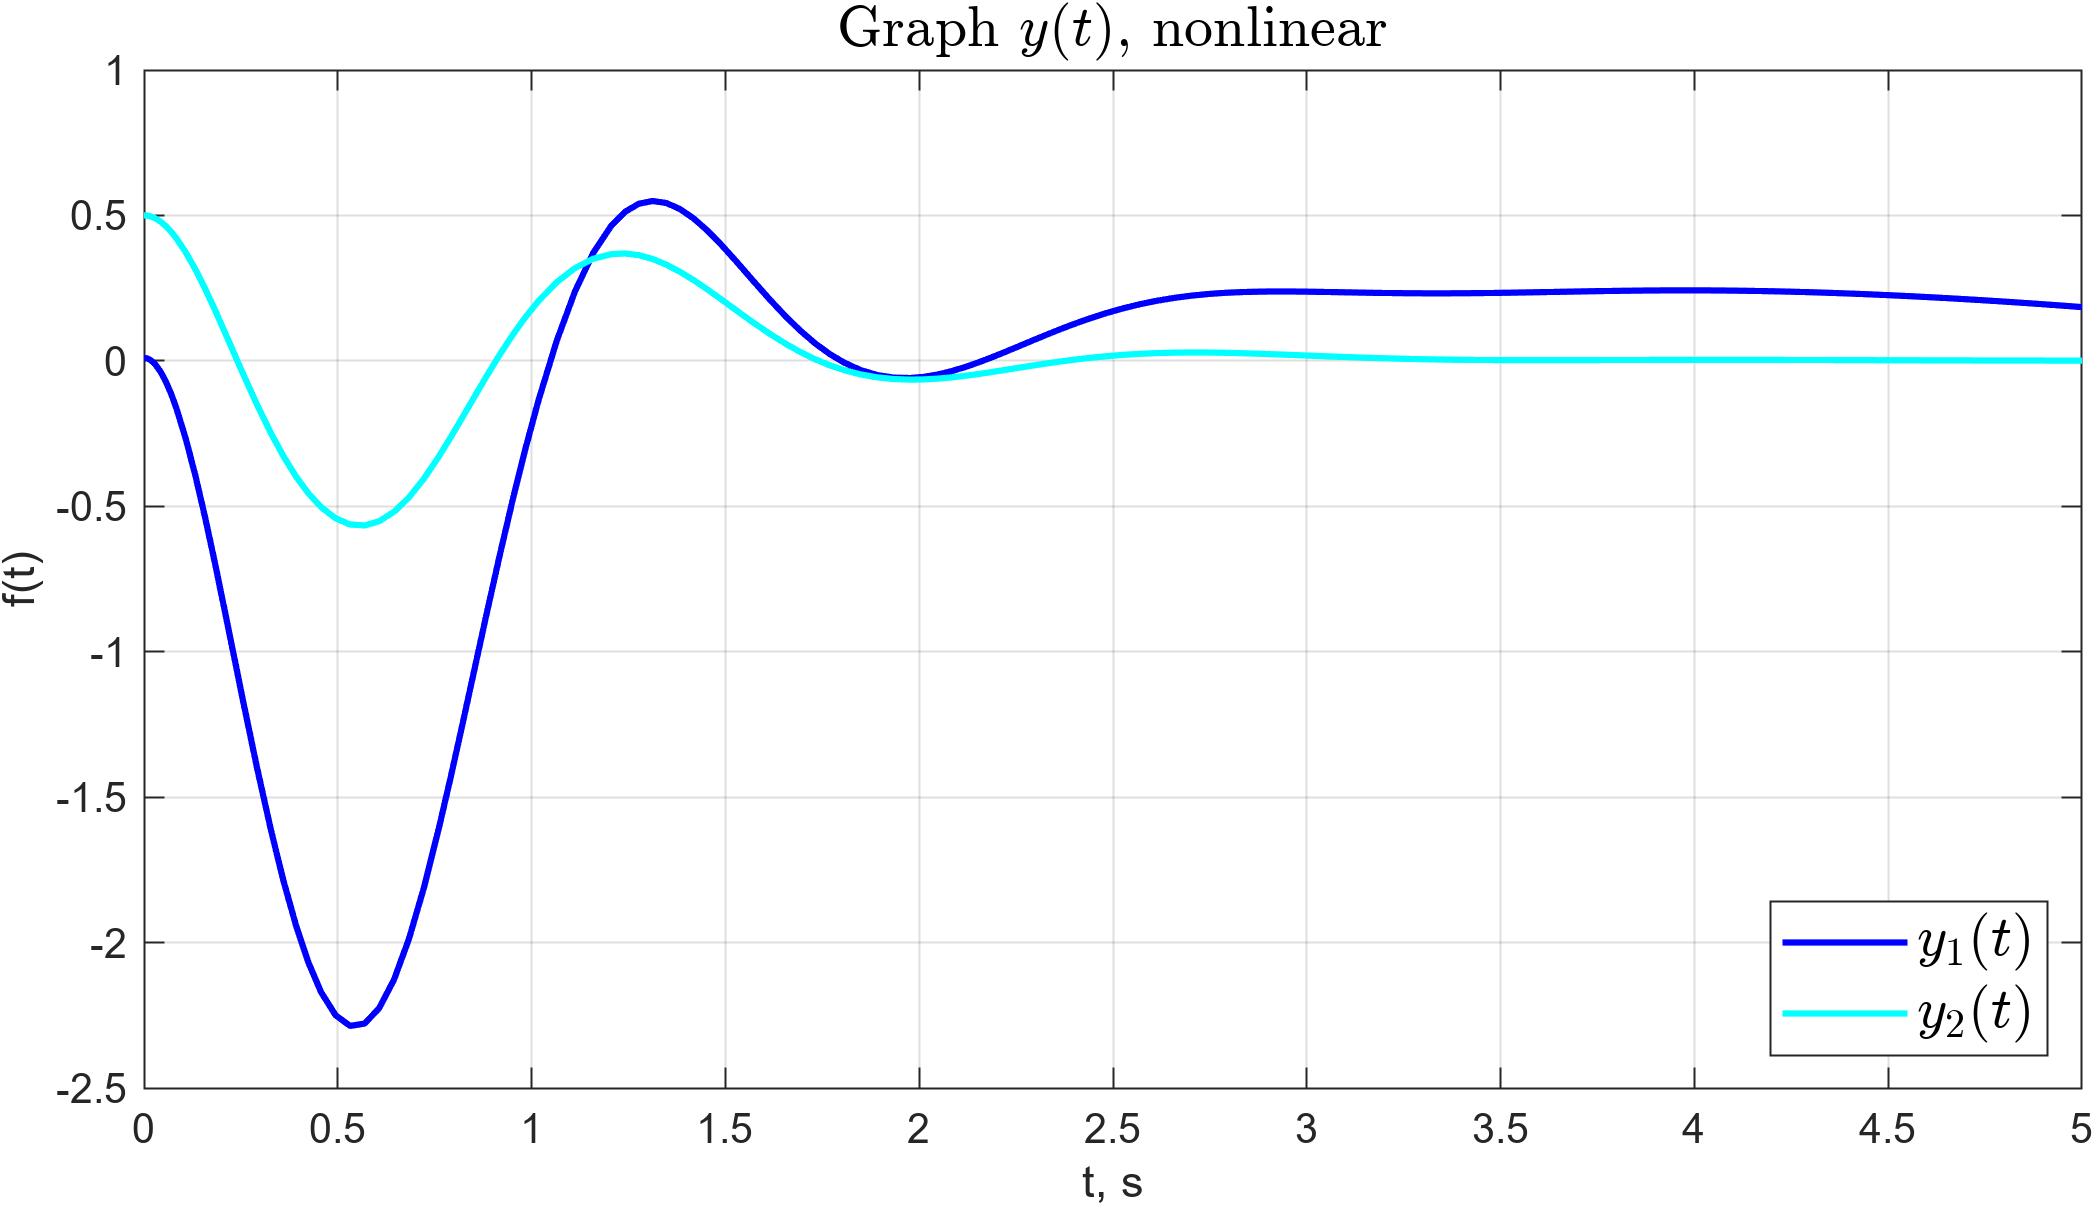
\includegraphics[width=1\linewidth]{pic2/5_f_nonlin_1.png}}
\caption{График выходного сигнала $y(t)$ для нелинейной системы при $x(0) = 
    [0.01 \,\, 0.01 \,\, 0.5 \,\, 0.01]^T$.}
\label{5_f_nonlin_1}
\end{figure}

При увеличении начального значения угла отклонения амплитуда $y_2(t)$ и время, за которое он сходится к нулю возрастает (рисунок \ref{5_f_nonlin_1}). Кроме того, не удается получить результаты моделирования при задании больших значений начального угла  за ограниченное время.





\section{Решение задачи слежения}

Пусть $f=0$. Зададимся целевым сигналом $g(t)$, который описывает желаемое поведение $\varphi (t)$

\begin{equation}
	g(t) = \sum \limits_{k=1}^5 A_k \sin(\omega_kt+\phi_k),
\end{equation}
где
\begin{equation}
	\begin{matrix}
		A_1 = 1, & \omega_1 = 0.5, & \phi_1 = 0\\
		A_2 = 0.8, & \omega_2 = 1, & \phi_2 = \pi /4\\
		A_3 = 0.6, & \omega_3 = 1.5, & \phi_3 = \pi /3\\
		A_4 = 0.4, & \omega_4 = 2, & \phi_4 = -\pi/4\\
		A_5= 0.2, & \omega_5 = 2.5, & \phi_5 = \pi / 6\\
	\end{matrix}
\end{equation}

Построим следящий регулятор, гарантирующий выполнение условия

\begin{equation}
	\lim \limits_{t\to \infty} \| \varphi (t) - g(t) \| = 0
\end{equation}

Запишем целевой сигнал $g$ через генератор

\begin{equation}
\begin{cases}
	\dot{w}_g = \Gamma_g w_g\\
	g = Y_g w_g
\end{cases}
\end{equation}

Значения матриц $\Gamma_g$, $Y_g$, $w_g(0)$ совпадают соответственно с $\Gamma_f$, $Y_f$, $w(0)$, так как сигналы $g(t)$ и $f(t)$ одинаковы.

Необходимый регулятор будет иметь вид

\begin{equation}
	u = Kx + K_g w_g
\end{equation}

Стабилизирующую компоненту $K$ выберем такой же как и в прошлом пункте. 
Запишем систему уравнений Франкиса-Дэвисона

\begin{equation}
	\begin{cases}
		P_g \Gamma_g - (A+BK) P_g = BK_g\\
		CP_g = Y_g
	\end{cases}
\end{equation}

Условие существование здесь будет то же, что и в прошлом пункте.

Синтезируем матрицу следящей компоненты регулятора

\begin{equation}
	K_g = \begin{bmatrix}
		-83795\\	-101630\\	-28825\\	15476\\	-4671\\	13280\\	-6636.1\\	-1338.9\\	-280.4743\\	2710.3
	\end{bmatrix}^T
\end{equation}

И выполним моделирование для линейной системы

\begin{figure}[!h]
	\center{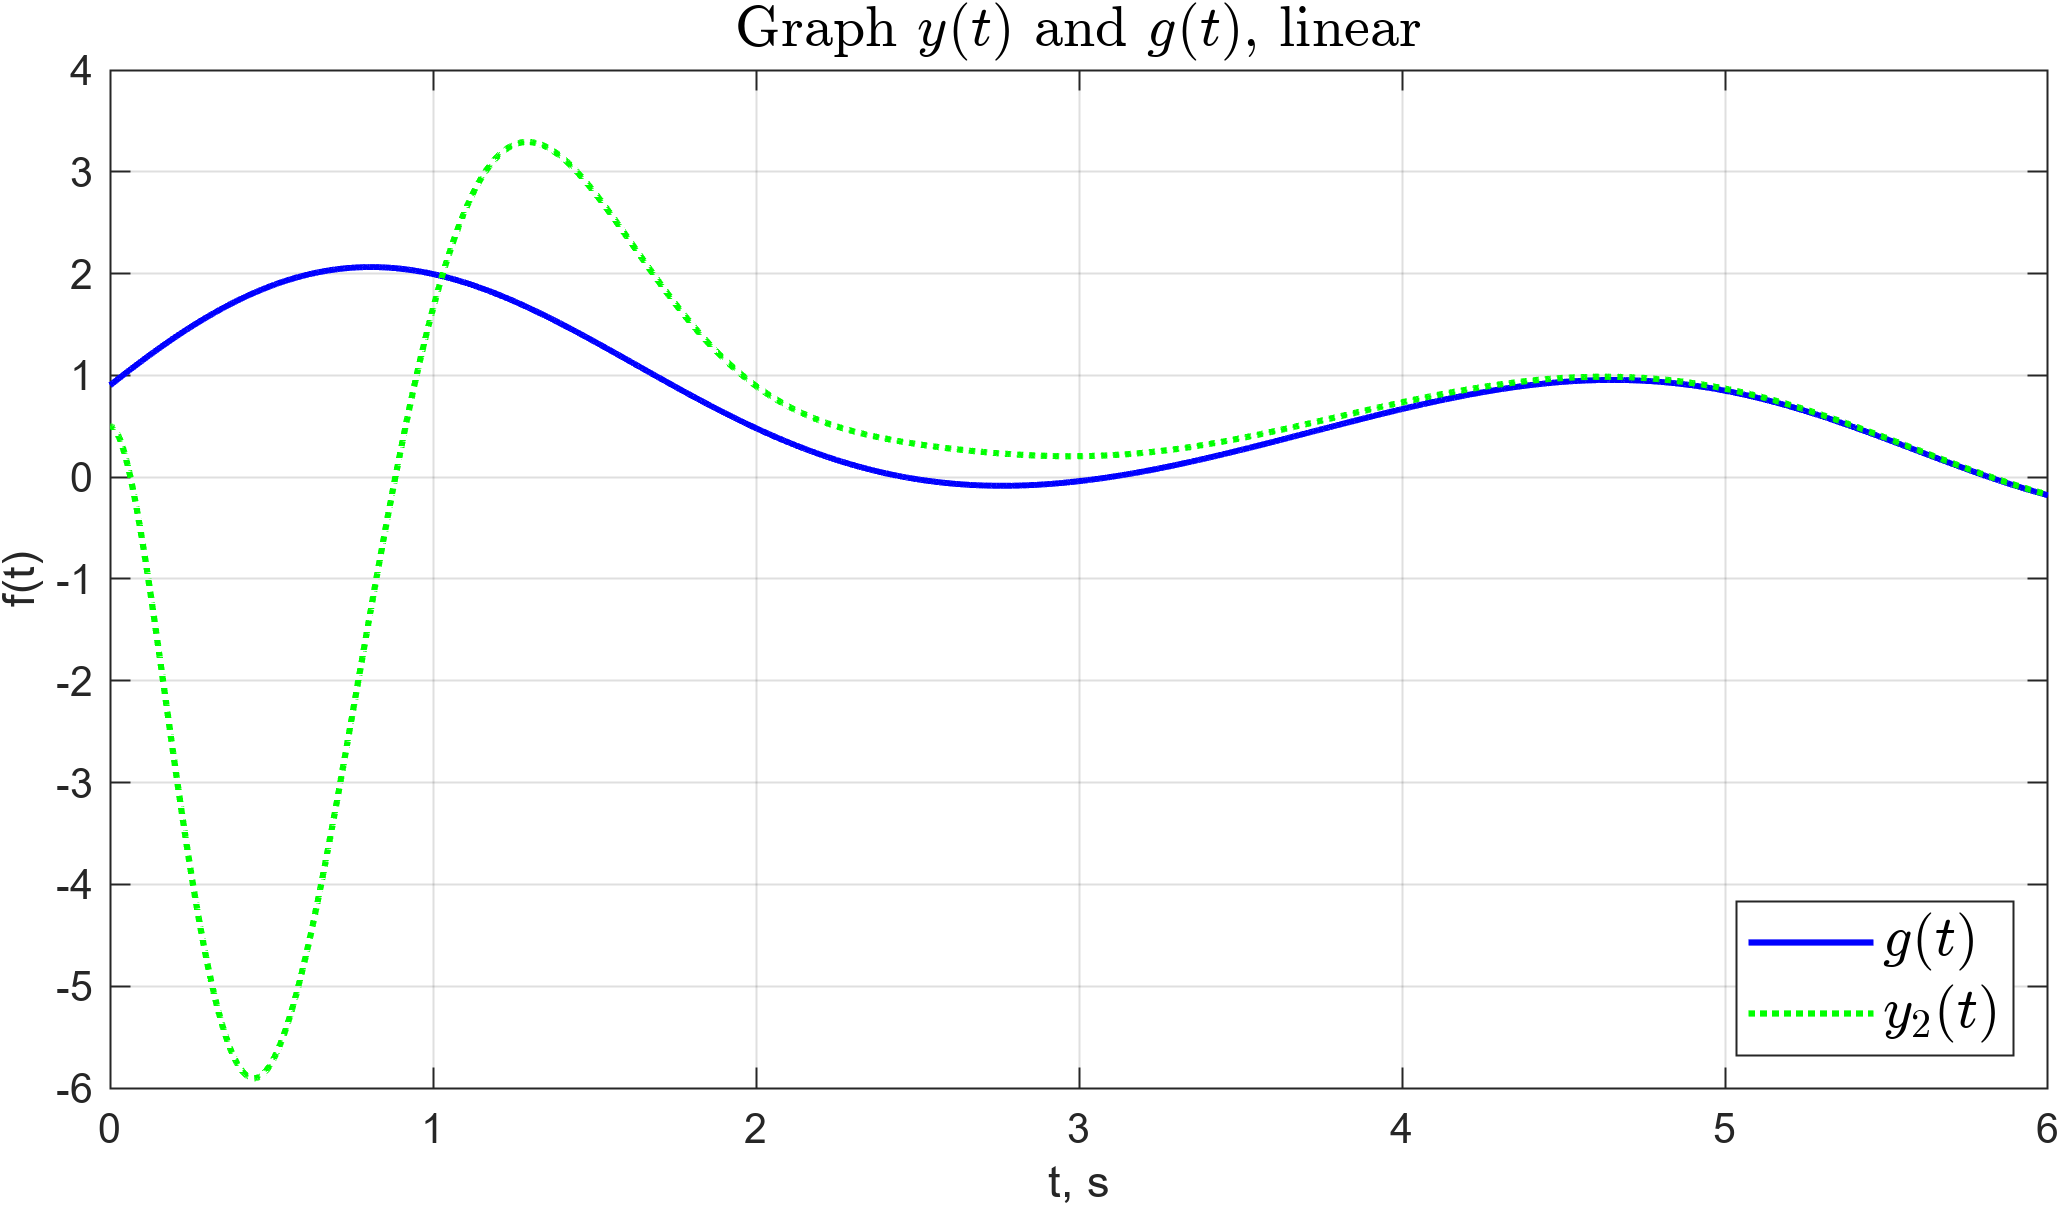
\includegraphics[width=1\linewidth]{pic2/5_g_lin.png}}
	\caption{Графики выходного сигнала $y_2(t)$ и задающего сигнала $g(t)$ для линейной системы.}
	\label{5_g_lin}
\end{figure}

\begin{figure}[!h]
	\center{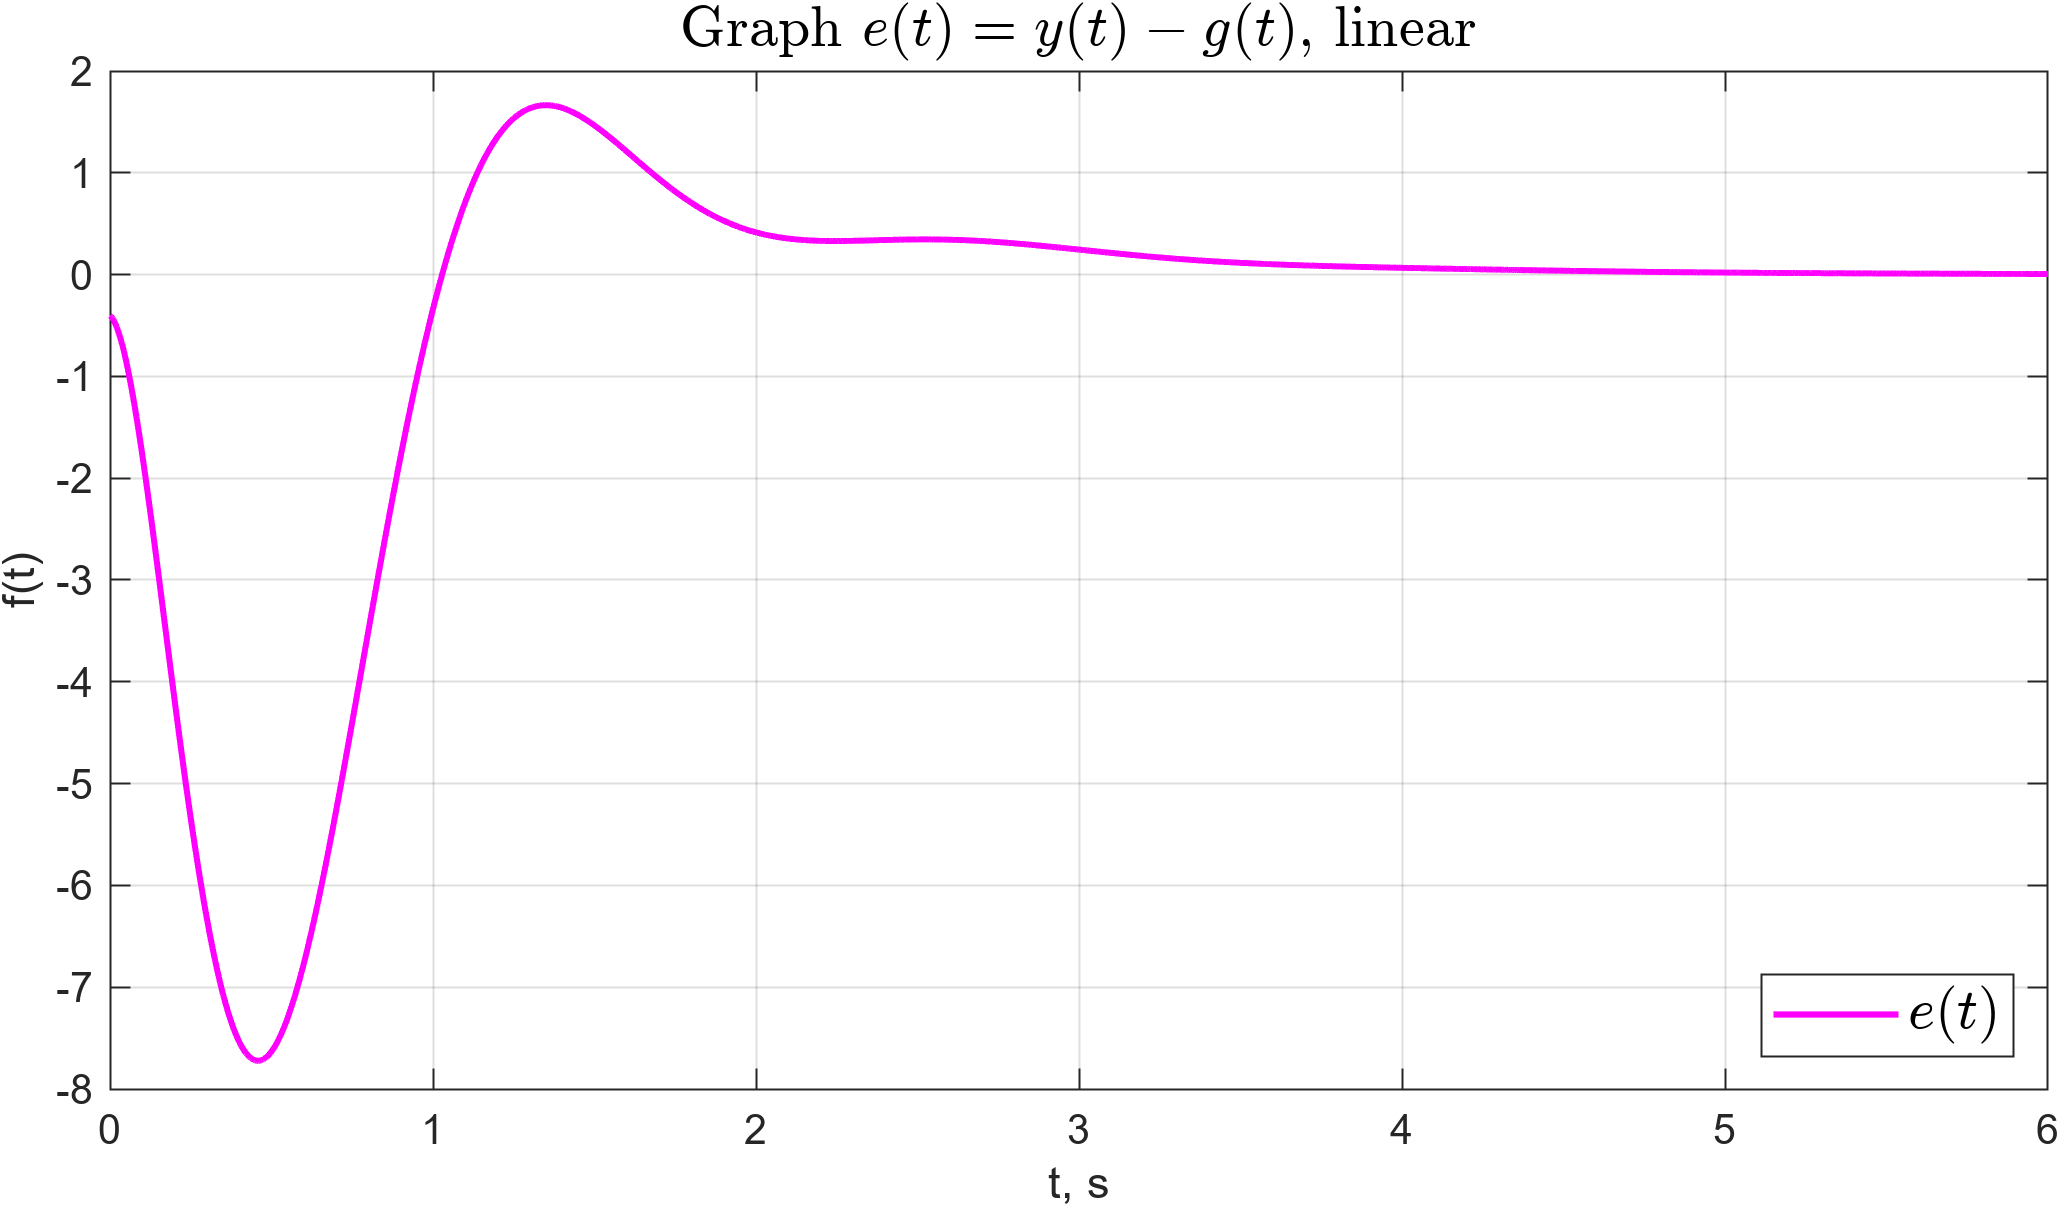
\includegraphics[width=1\linewidth]{pic2/5_e_lin.png}}
	\caption{График ошибки слежения $e(t) = y_2(t)-g(t)$ для линейной системы.}
	\label{5_e_lin}
\end{figure}

Как видно из рисунков \ref{5_e_lin} и \ref{5_g_lin} задача слежения для линейной системы с помощью синтезированного регулятора выполнена.


Перейдем к моделированию работы регулятора в случае нелинейной системы.  

\begin{figure}[!h]
	\center{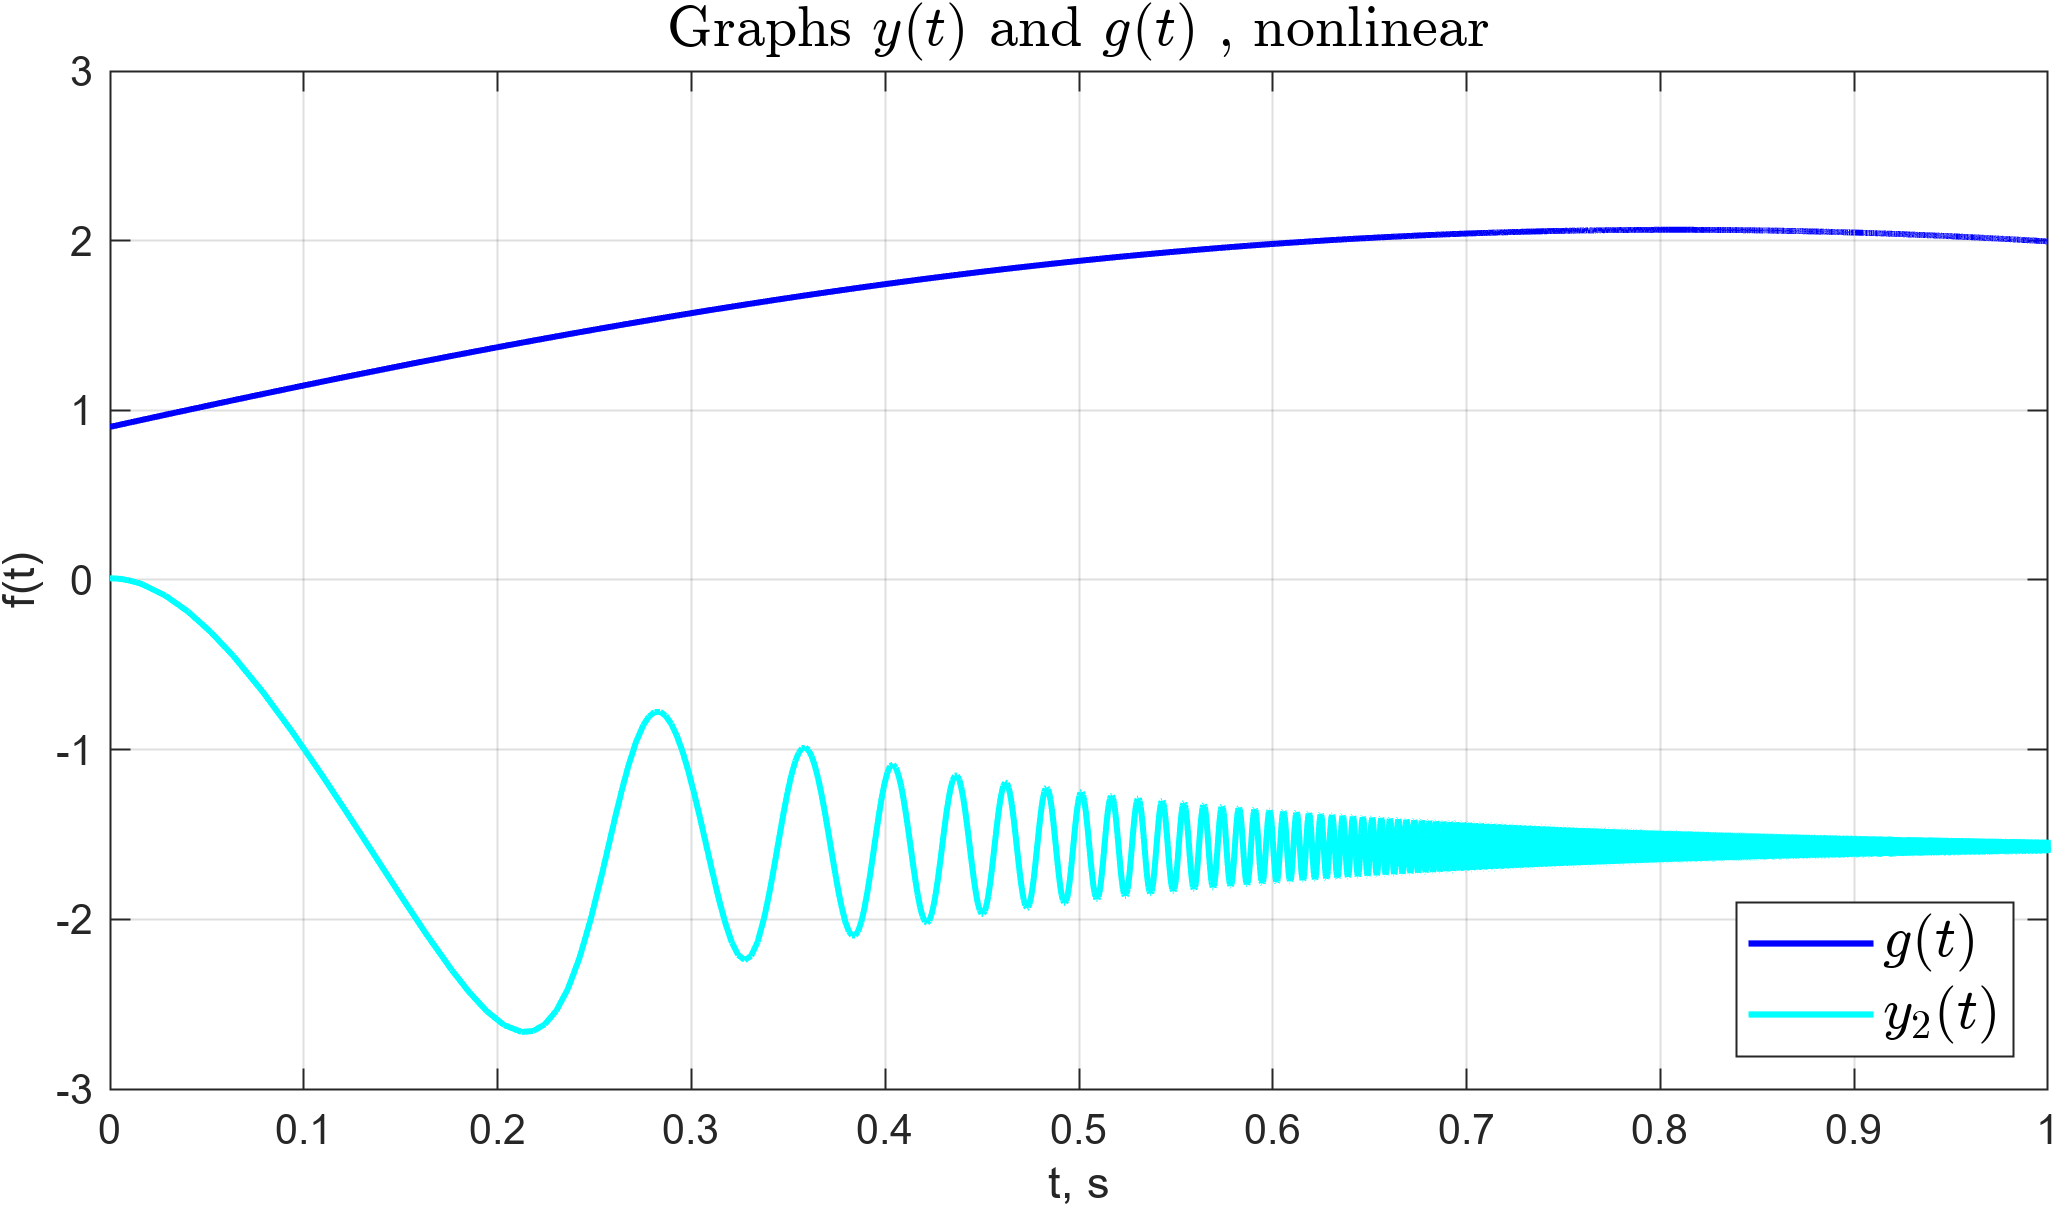
\includegraphics[width=1\linewidth]{pic2/5_g_nonlin.png}}
	\caption{Графики выходного сигнала $y_2(t)$ и задающего сигнала $g(t)$ для нелинейной системы.}
	\label{5_g_nonlin}
\end{figure}

Как можно заметить, задача слежения с использванием данного регулятора для нелинейной системы не решена. Возможно, значения $K_g$ оказались слишком большими по модулю. Попробуем подобрать другой регулятор. Из пункта 4.3 возьмем матрицу регулятора $$K = \begin{bmatrix}
4.5 & 49 & -3219 & -1334
\end{bmatrix}$$

Соответствующая матрица следящей компоненты

$$K_g = \begin{bmatrix}
	-336.6\\	234.0905\\	447.1551\\	-422.7219\\	191.4115\\	-966.0481\\	1013.6\\	264.1078\\	272.1893\\	-701.2038
\end{bmatrix}^T$$

График для данного варианта регулятора представлен на рисунке \ref{5_g_nonlin_1}.
\begin{figure}[!h]
	\center{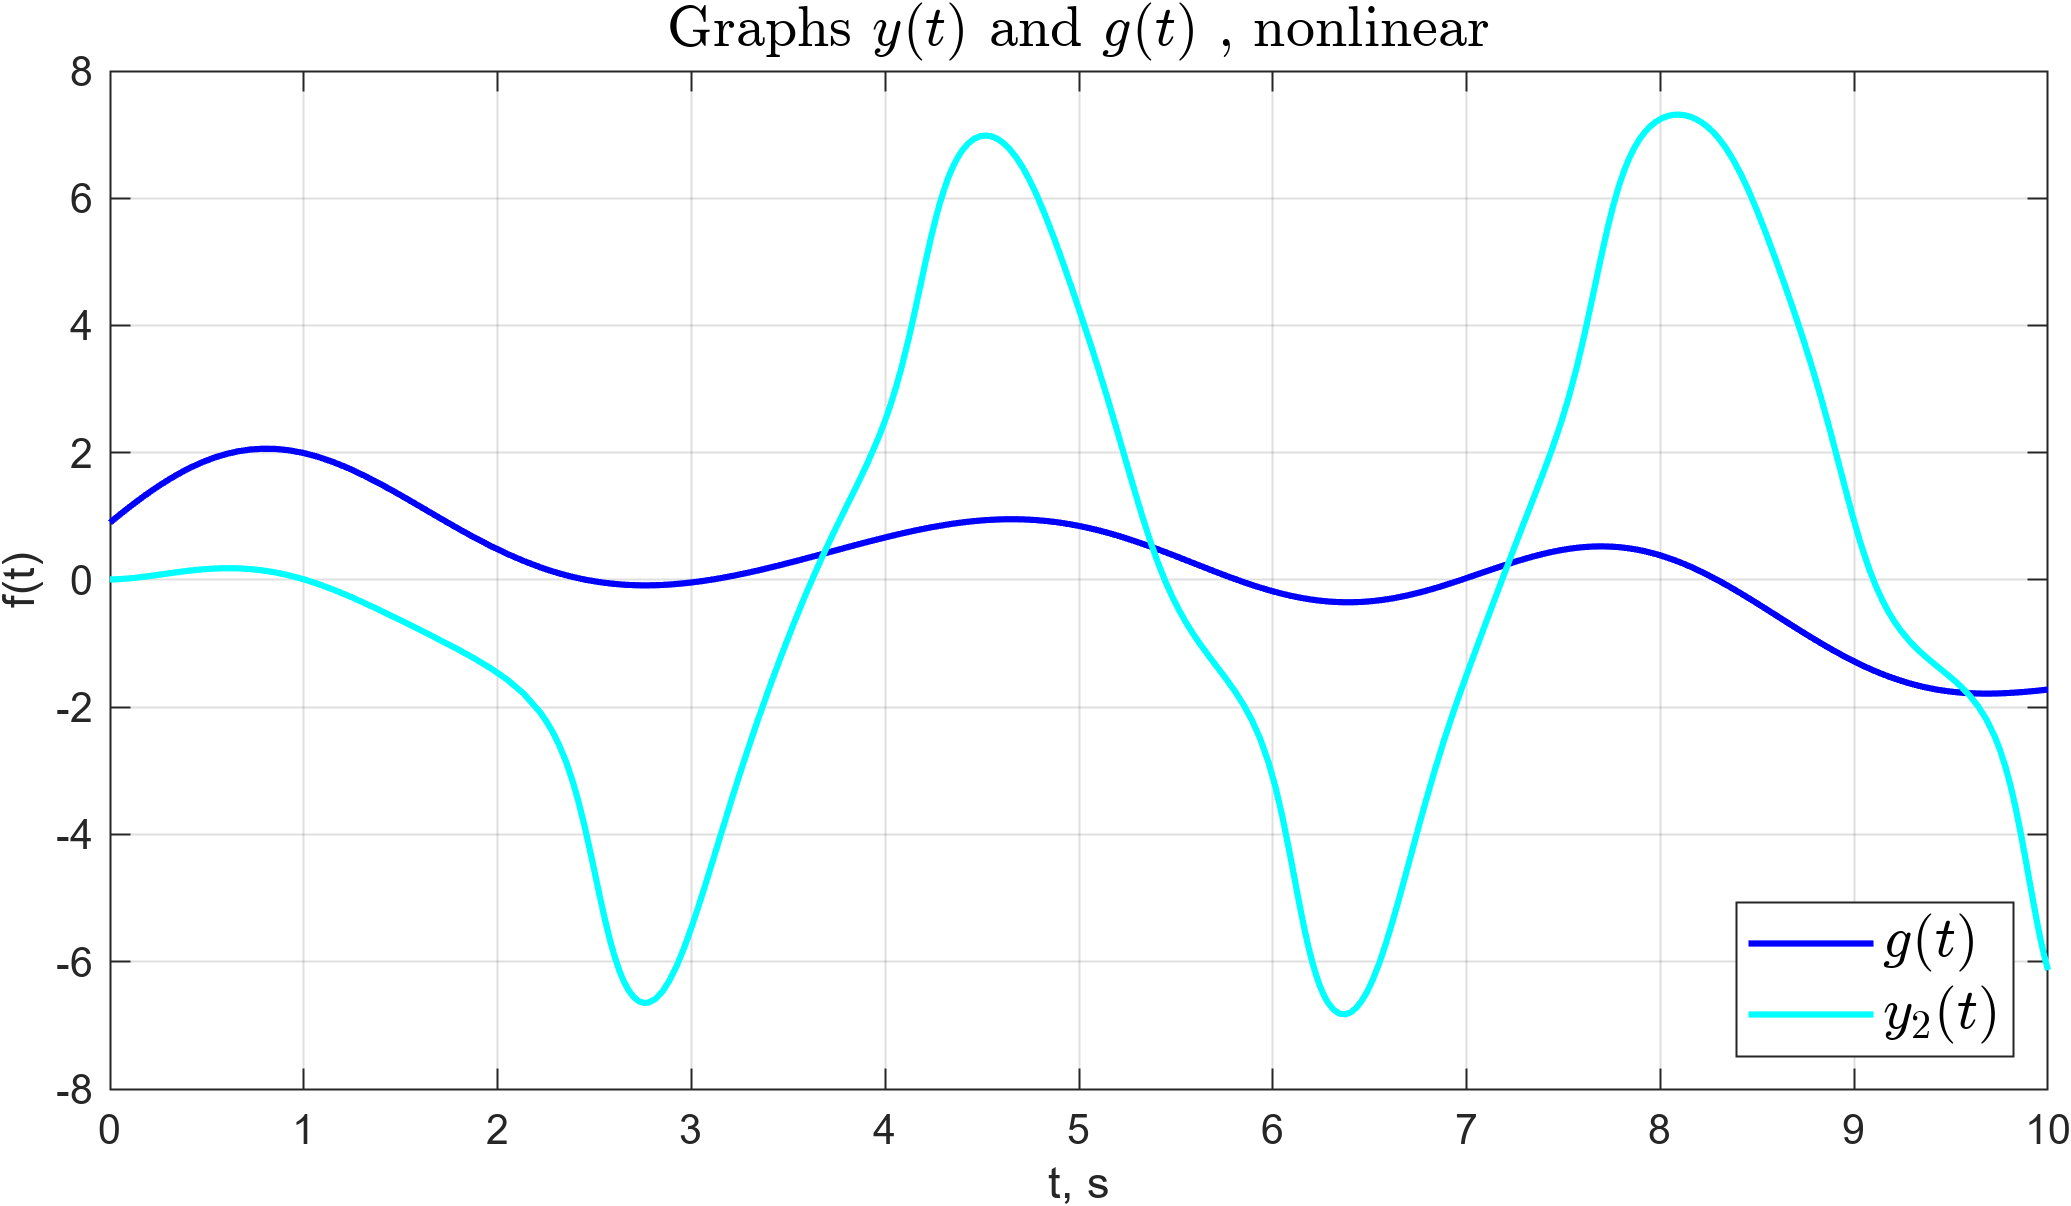
\includegraphics[width=1\linewidth]{pic2/5_g_nonlin_1.png}}
	\caption{Графики выходного сигнала $y_2(t)$ и задающего сигнала $g(t)$ для нелинейной системы.}
	\label{5_g_nonlin_1}
\end{figure}

\begin{figure}[!h]
	\center{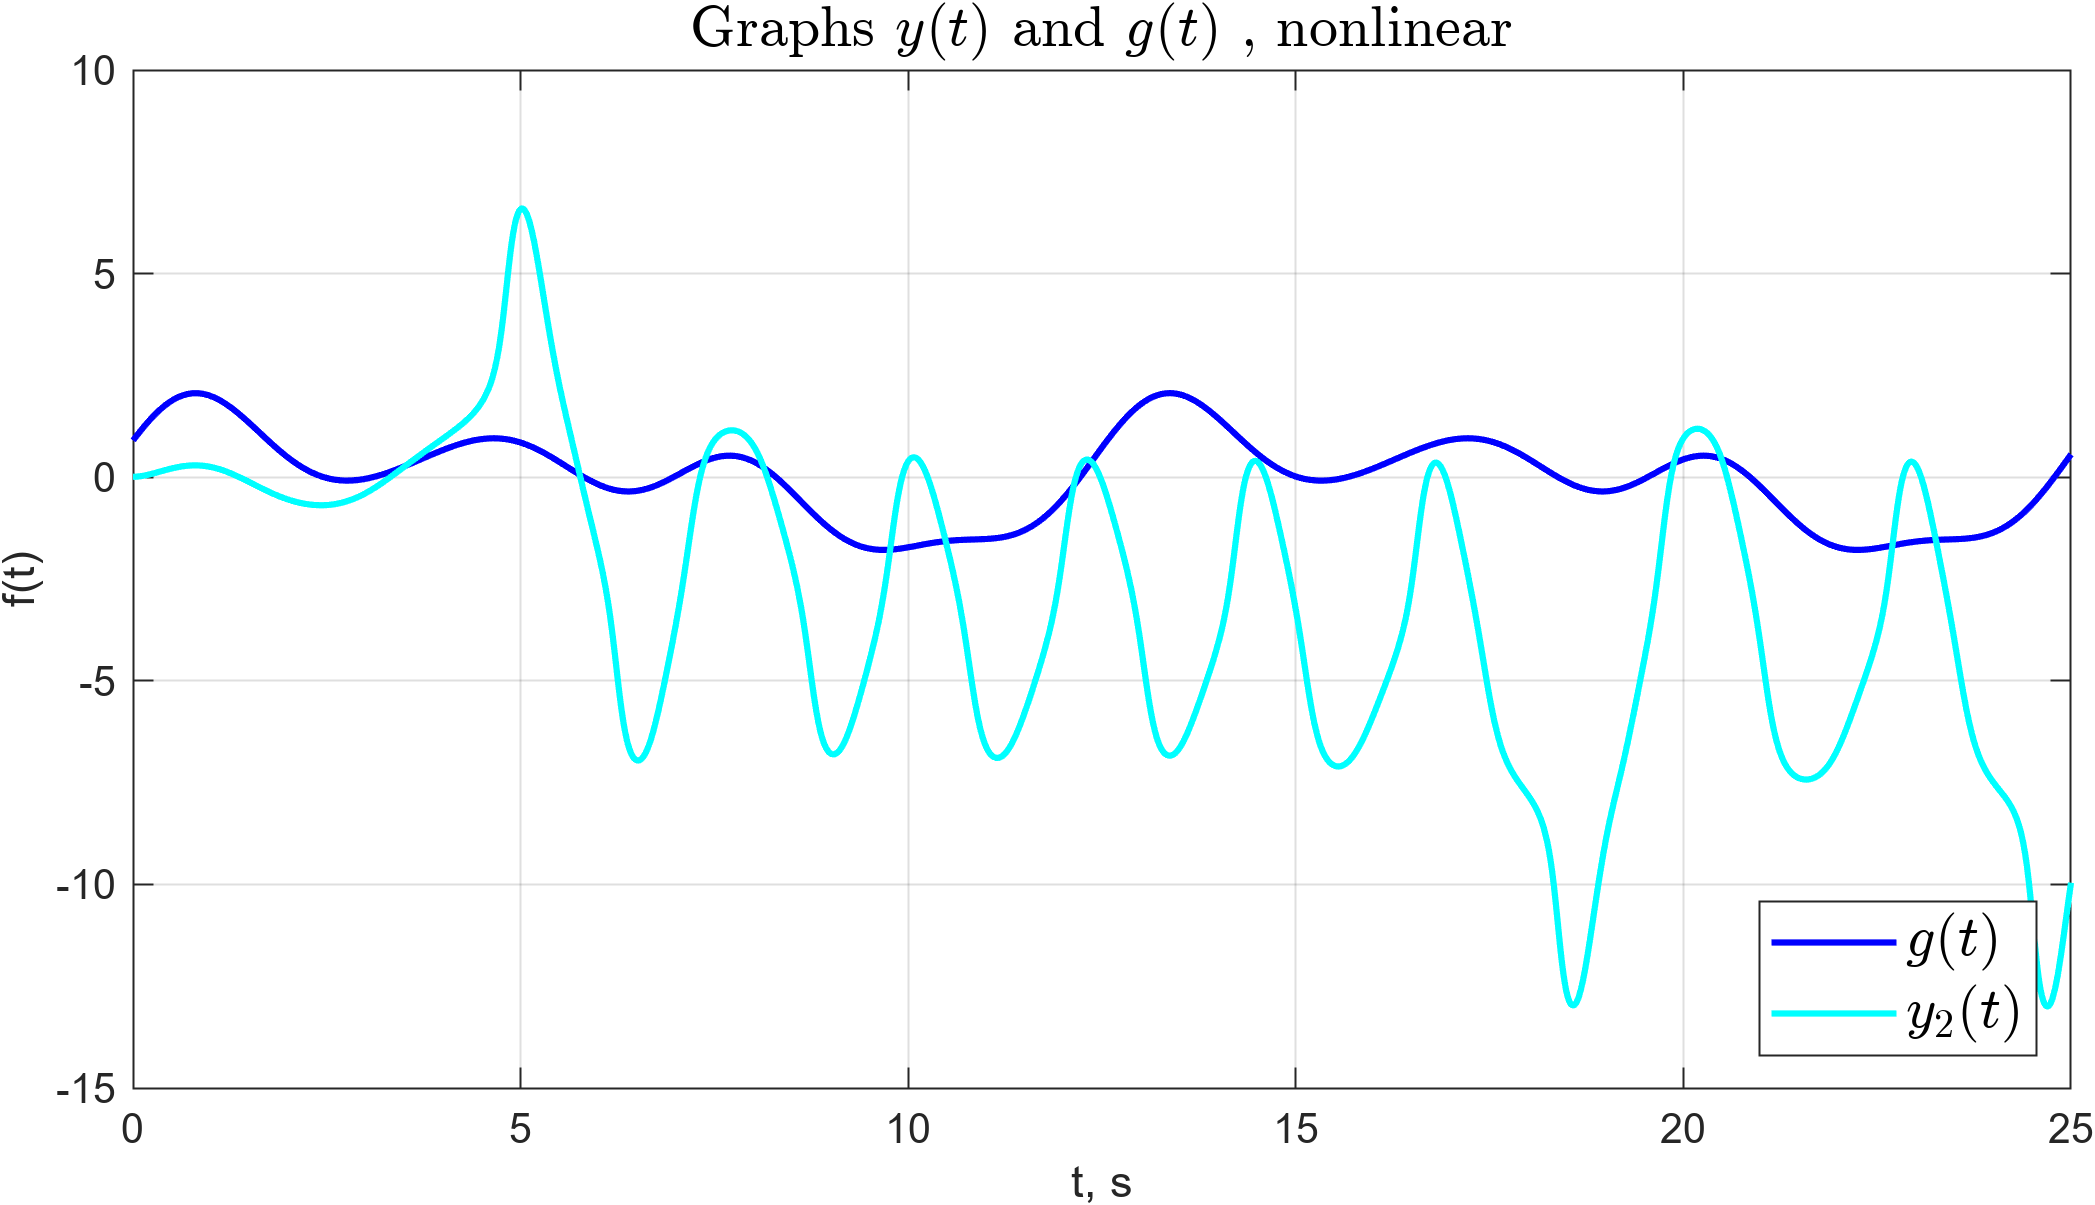
\includegraphics[width=1\linewidth]{pic2/5_g_nonlin_2.png}}
	\caption{Графики выходного сигнала $y_2(t)$ и задающего сигнала $g(t)$ для нелинейной системы.}
	\label{5_g_nonlin_2}
\end{figure}

На рисунке \ref{5_g_nonlin_2} представлен результат моделирования системы при 
\begin{equation}
	K = \begin{bmatrix}
		10.7930& 127.0276& -4567.3 &-1894.6
	\end{bmatrix}
\end{equation}
и соответственно
\begin{equation}
	K_g = \begin{bmatrix}
		-1654.4\\	1324.6\\	976.8675\\	490.8794\\	910.7887\\	-640.0242\\	772.5327\\	770.8408\\	536.4382\\	-547.1769
	\end{bmatrix}^T
\end{equation}


Для рассмотренных вариантов следящих регуляторов не удалось решить задачу слежения для нелинейной системы для заданного сигнала $g(t)$. Возможно, для данной системы необходимо применять другие подходы к синтезу следящих регуляторов. Либо подбирать другие базовые параметры системы: массу тележки и маятника, например или менять гармоники сигнала $g(t)$. 

Попробуем решить задачу слежения для сигнала $\tilde{g}(t)$

\begin{equation}
	\tilde{g}(t) = \sum \limits_{k=1}^5 A_k \sin(\omega_kt+\phi_k),
\end{equation}
где
\begin{equation}
	\begin{matrix}
		A_1 = 0.1, & \omega_1 = 1, & \phi_1 = 0\\
		A_2 = 0.08, & \omega_2 = 2, & \phi_2 = \pi /4\\
		A_3 = 0.06, & \omega_3 = 3, & \phi_3 = \pi /3\\
		A_4 = 0.04, & \omega_4 = 4, & \phi_4 = -\pi/4\\
		A_5= 0.02, & \omega_5 = 5, & \phi_5 = \pi / 6\\
	\end{matrix}
\end{equation}

Выберем матрицу  $$K = \begin{bmatrix}
3064& 4364& -26684& -11174
\end{bmatrix}$$

Синтезируем матрицу следящей компоненты регулятора

\begin{equation}
	K_g = \begin{bmatrix}
		-3915.7\\	-1179.9\\	-267.7877\\	1327.2\\	484.7377\\	509.1376\\	-157.5224\\	378.8155\\	228.299\\	7.1794
	\end{bmatrix}^T
\end{equation}

И выполним моделирование для линейной (рисунки и ) и нелинейной систем (рисунки \ref{5_g_nonlin_another} и \ref{5_g_nonlin_another_e}), начальные условия $x(0) = 
[0.01 \,\, 0.01 \,\, 0.01 \,\, 0.01]^T$. Заметим, что в обоих случаях задача слежения успешно выполнена.


\begin{figure}[!h]
	\center{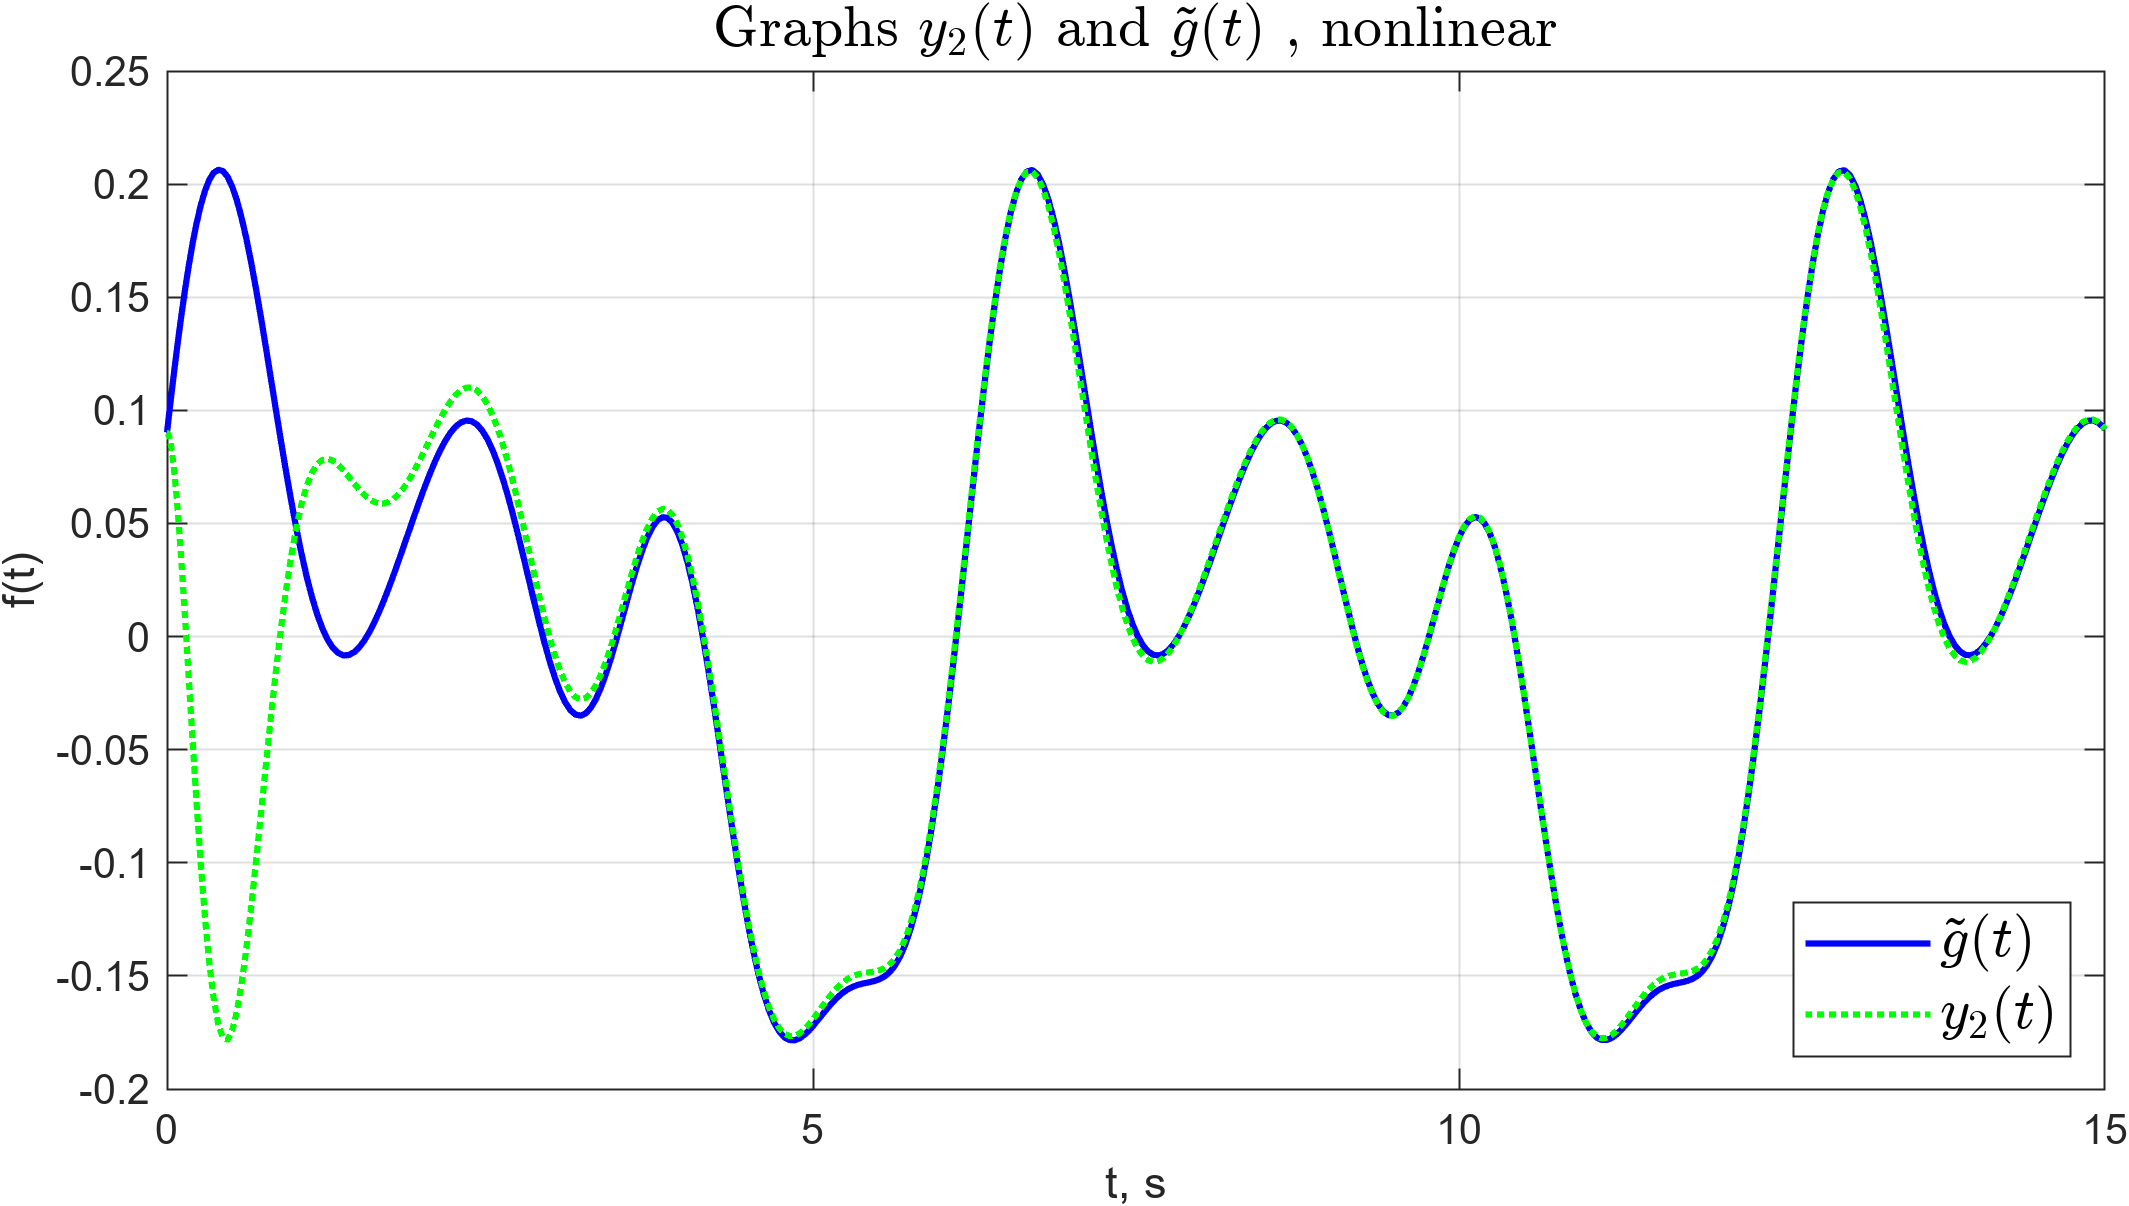
\includegraphics[width=1\linewidth]{pic2/5_g_nonlin_another.png}}
	\caption{Графики выходного сигнала $y_2(t)$ и задающего сигнала $\tilde{g}(t)$ для нелинейной системы.}
	\label{5_g_nonlin_another}
\end{figure}

\begin{figure}[!h]
	\center{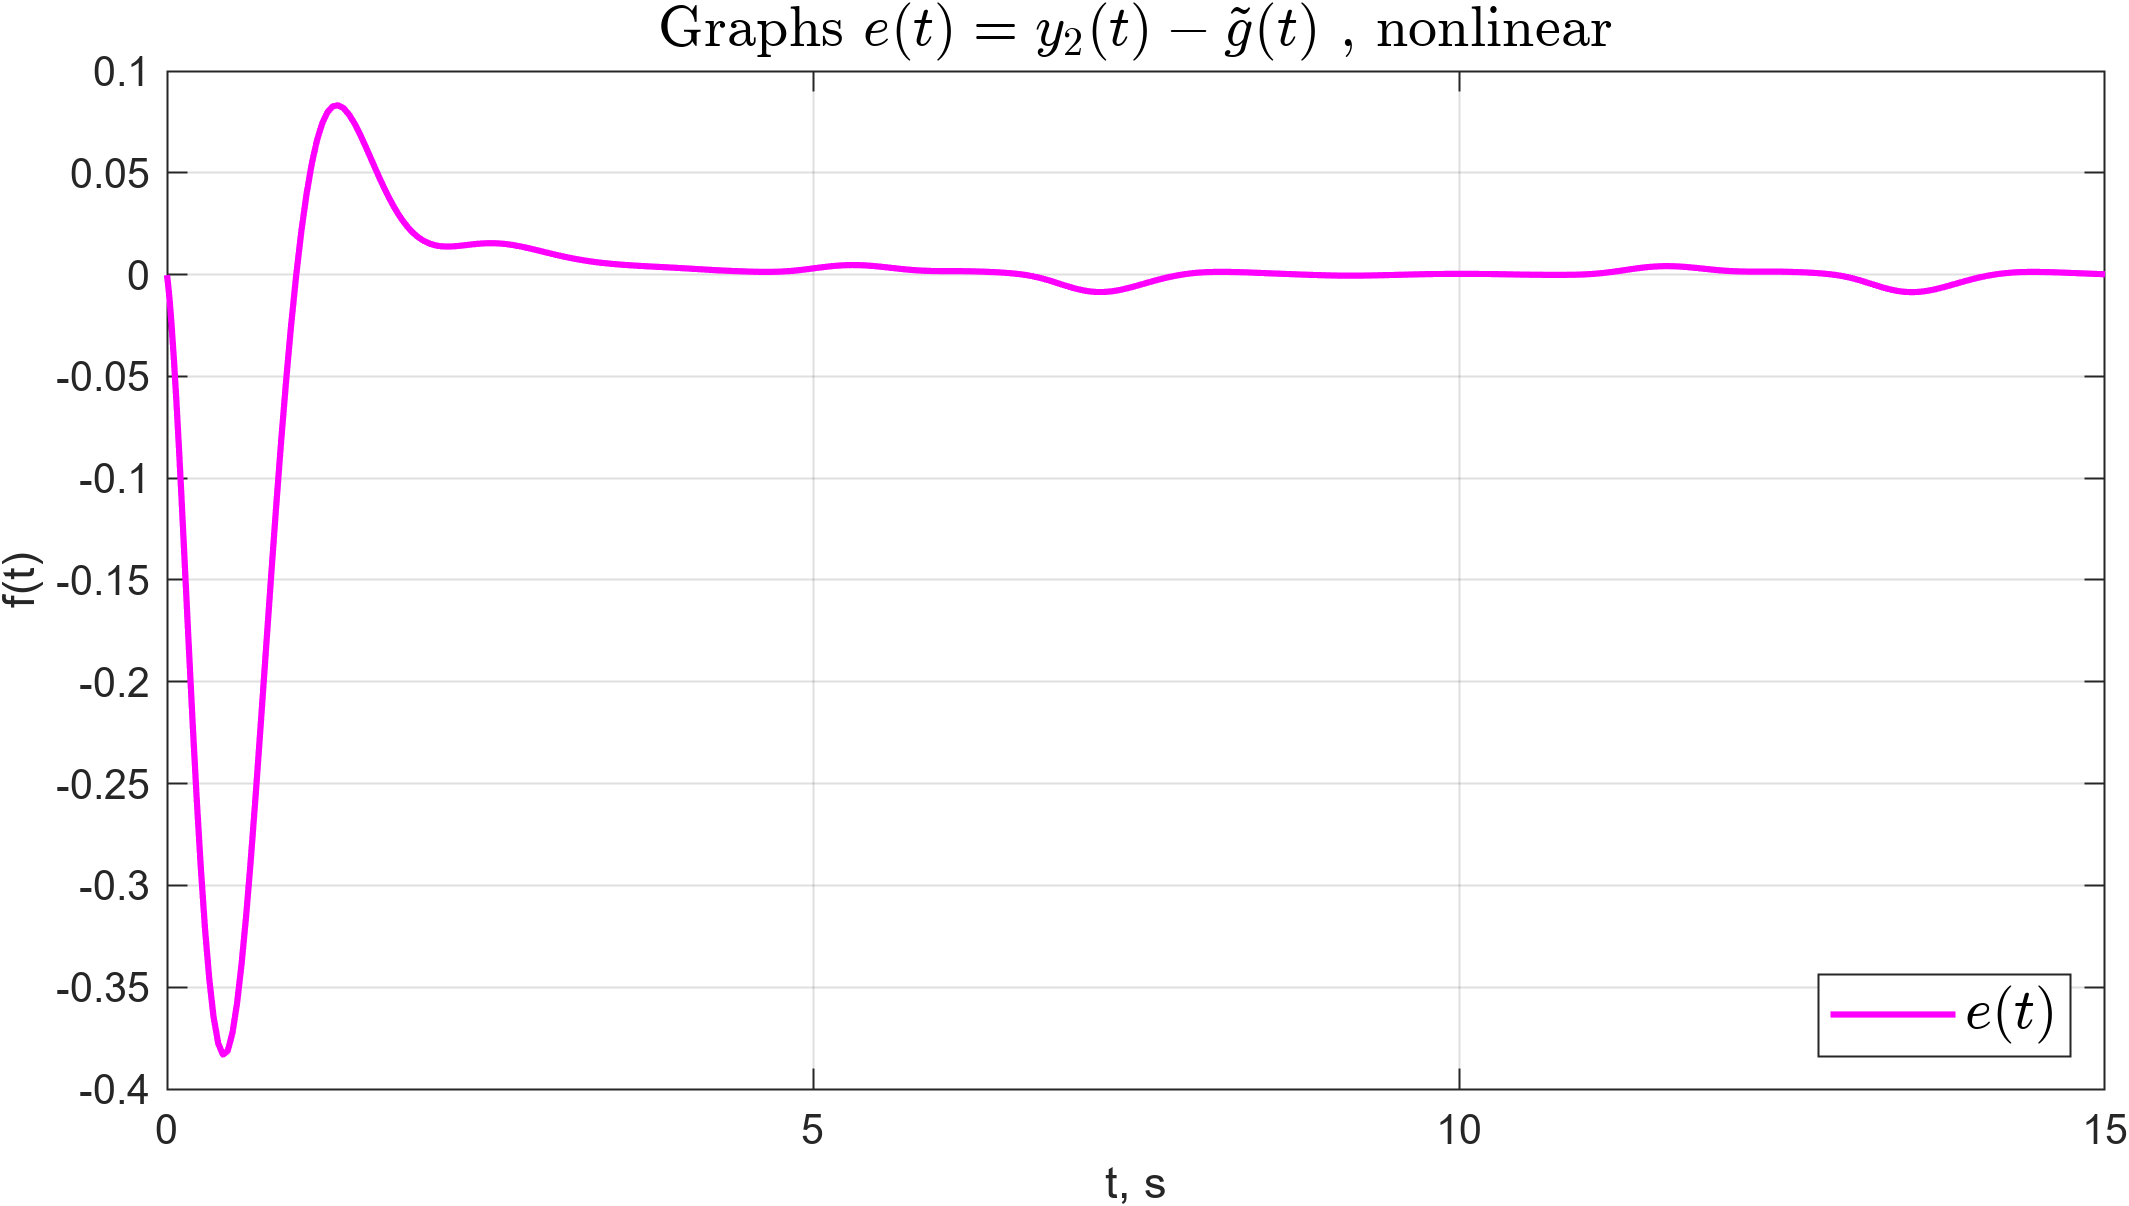
\includegraphics[width=1\linewidth]{pic2/5_g_nonlin_another_e.png}}
	\caption{График ошибки слежения $e(t) = y_2(t)-\tilde{g}(t)$ для нелинейной системы.}
	\label{5_g_nonlin_another_e}
\end{figure}



\endinput